%======================================================================
\NEWSEC
%======================================================================

\subsection{\ssAdapt}

%----------------------------------------------------------------------

\begin{frame}[fragile,label=ss-adapt] 
\secframetitle{\ssAdapt}
\bluebf{Mesh refinement proceeds in several steps}

\begin{enumerate}
\item Apply refinement criteria (\code{Refine})
\item Tell neighbor \code{Block}s your desired level
\begin{itemize}
\item \code{Block}s form a chare array
\item remote entry method call to neighbor blocks
\end{itemize}
\item Receive neighbor level
\begin{itemize}
\item entry method
\item called by neighbors
\end{itemize}
\item Update own level if needed (goto \bluebf{2})
\item Exit after \blueit{quiescence}
\begin{itemize}
\item no processor is executing an entry point
\item no messages are awaiting processing
\item and no messages in-flight
\end{itemize}
\end{enumerate}
\end{frame}

%----------------------------------------------------------------------

\begin{frame}[fragile]
\secframetitle{\ssAdapt}
\begin{center}
\begin{minipage}{3in}
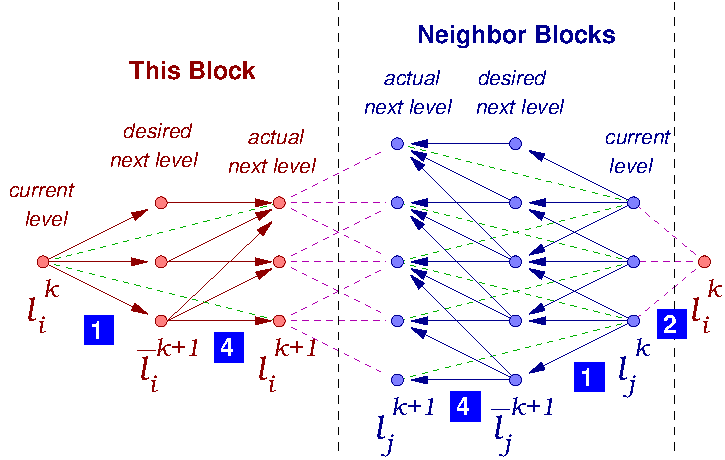
\includegraphics[width=3in]{amr-2.pdf}
\end{minipage}
\end{center}
\pause
\begin{itemize}
\item \greentext{temporal level jump criterion}
\pause
\item \magentatext{spacial level jump criterion}
\end{itemize}
\end{frame}

%----------------------------------------------------------------------

\begin{frame}[fragile] 
\secframetitle{\ssAdapt}
\blockblue
\begin{center}
\begin{minipage}{2.5in}
\ANIMATEGRAPHICS{width=2.5in}{40}{Images/Circle/mesh-00}{475}{951}
\end{minipage}
\end{center}
\end{frame}
